% NWQMC.tex
\documentclass{beamer}
\usetheme{Boadilla}
\usepackage{amsmath}


\AtBeginSection[]
{
  \begin{frame}
    \frametitle{Table of Contents}
    \tableofcontents[currentsection]
  \end{frame}
}


% items enclosed in square brackets are optional; explanation below
\title[Surprise theory]{Bayesian surprise as a tool for monitoring sensor networks}
\author[W. Brooks]{Wesley Brooks}
\institute[USGS-WiWSC]{
  USGS Wisconsin Water Science Center\\
  and University of Wisconsin-Madison Department of Statistics\\
  Madison, WI\\[1ex]
  \texttt{wrbrooks@usgs.gov}
}
\date[May 2012]{May 3, 2012}

\begin{document}

%--- the titlepage frame -------------------------%
\begin{frame}[plain]
	\titlepage
	\vspace{-20mm}
	\begin{center}
		\includegraphics[width=0.3\textwidth]{../../figures/usgs-logo}
		\hspace{30mm}
		
\includegraphics[width=0.2\textwidth]{../../figures/bucky}
	\end{center}
\end{frame}

\begin{frame}{Table of Contents}
\tableofcontents
\end{frame}


\section{Overview}
%Huge amount of automated data collection that needs to be checked for quality assurance and control. Failures in remote sensor networks might go undetected until someone needs the data and can't get it. We need an automated method to identify changes in the data stream

\begin{frame}{Intro}
\end{frame}


\section{Background}
%History of the theory of Bayesian surprise: it was originally developed as a mimic for human attention for use in computer vision.

\subsection{Bayesian statistics}

\begin{frame}{Bayesian statistics}
	Bayesian statistics views a probability distribution as representing our degree of belief. This idea can be applied both to our data and to the underlying data-generating model.\\
	\vspace{3mm}
	\begin{itemize}
		\item Examples of the three distributions used in this work:
		\begin{itemize}
			\item $X \sim \text{Normal}(\mu=0, \tau=1)$
			\item $Y \sim \text{Gamma}(\alpha=2, \beta=1)$
			\item $Z \sim \text{t}_{\nu=4}(\mu=0, \sigma^2=1)$
		\end{itemize}
	\end{itemize}
	\begin{center}
		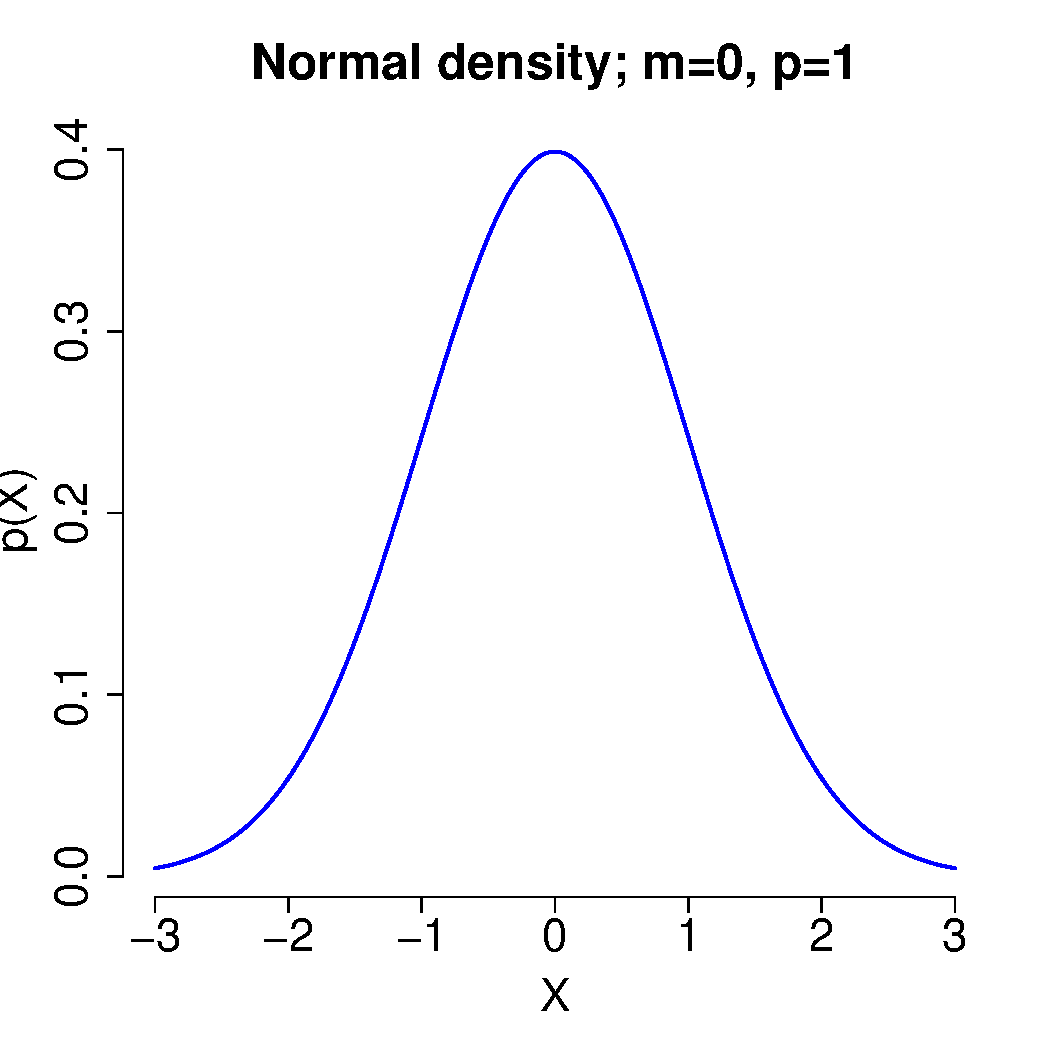
\includegraphics[width=0.33\textwidth]{../../figures/normal_pdf}
		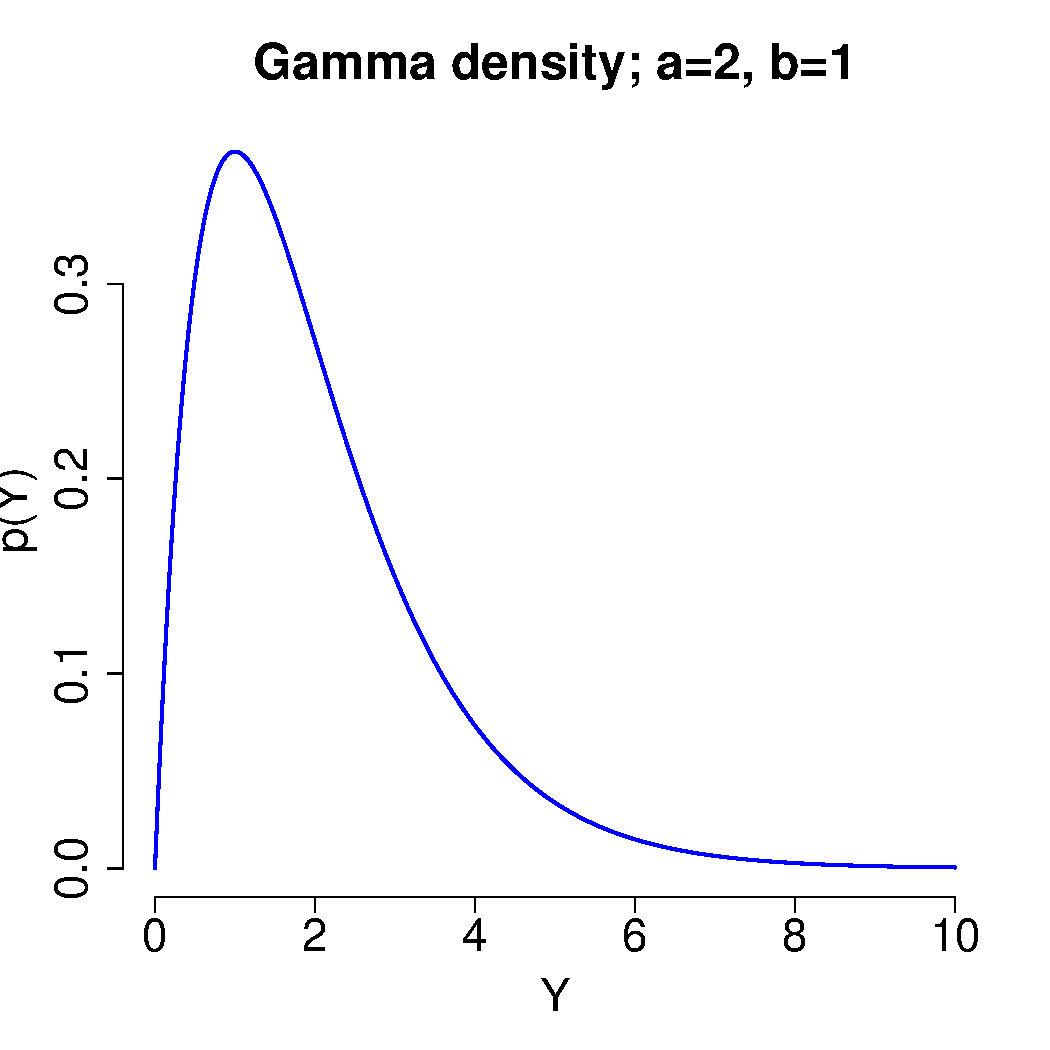
\includegraphics[width=0.33\textwidth]{../../figures/gamma_pdf}
		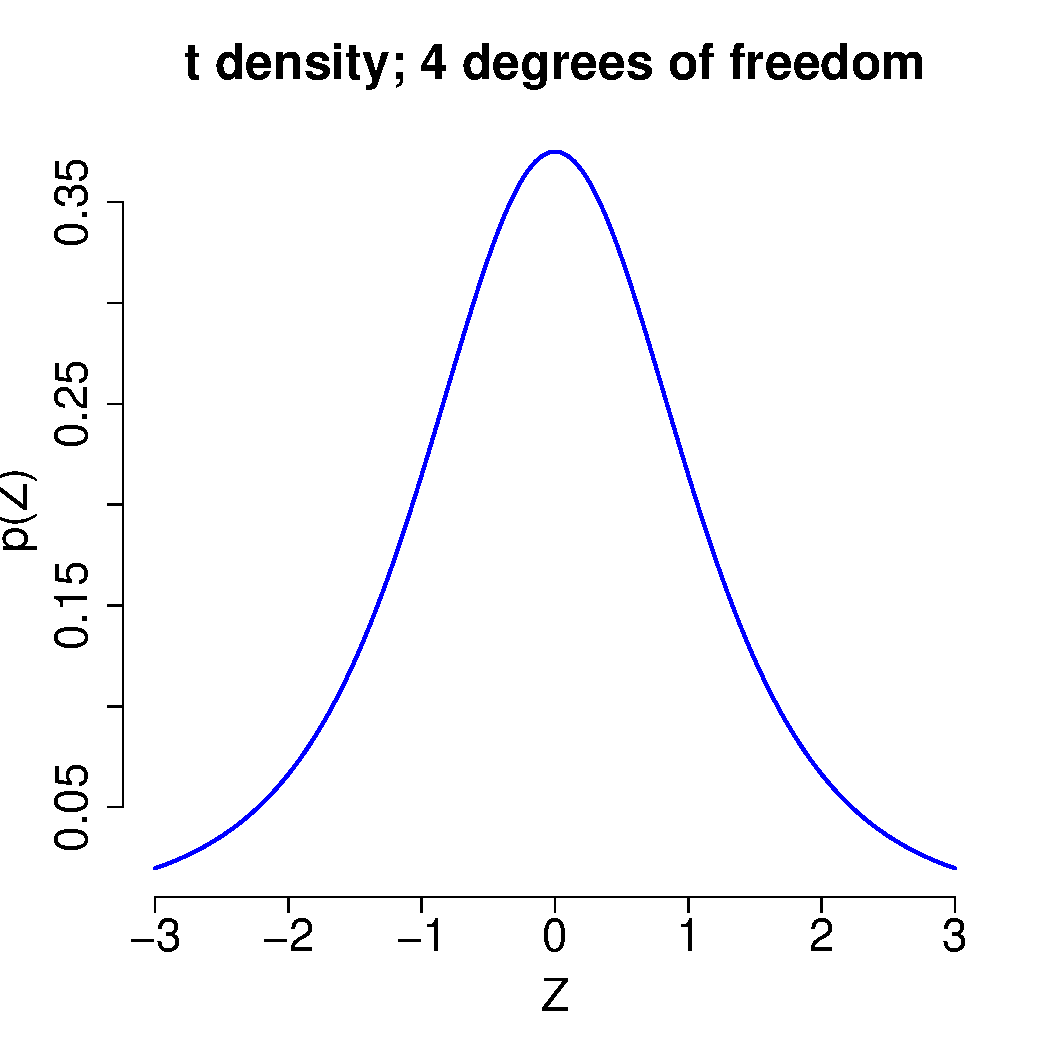
\includegraphics[width=0.33\textwidth]{../../figures/t_pdf}
	\end{center}
\end{frame}


\begin{frame}{Hierarchical models}
	\begin{itemize}
		\item A hierarchical model has more than one random element
		\item Randomness at one level feeds into the next
	\end{itemize}

	\begin{center}
		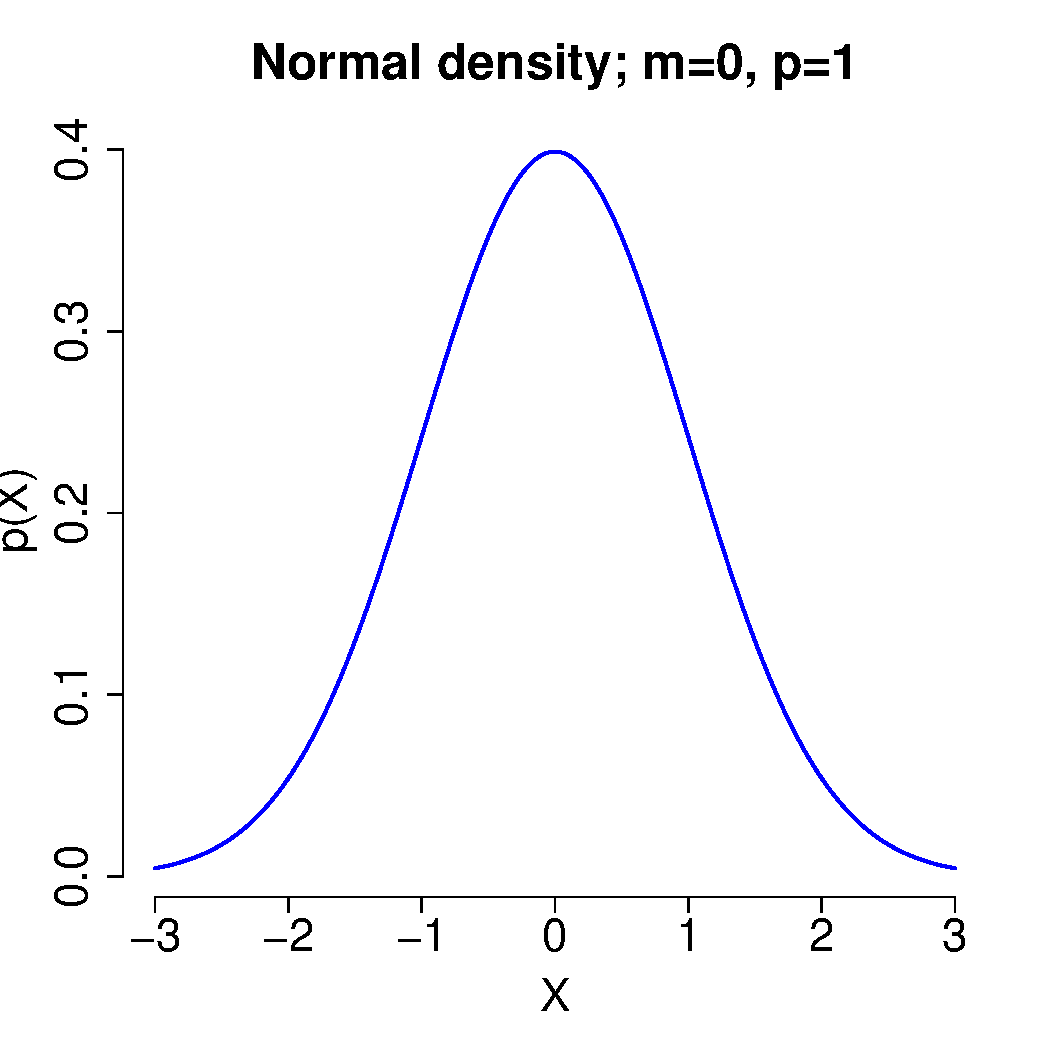
\includegraphics[width=0.33\textwidth]{../../figures/normal_pdf}
		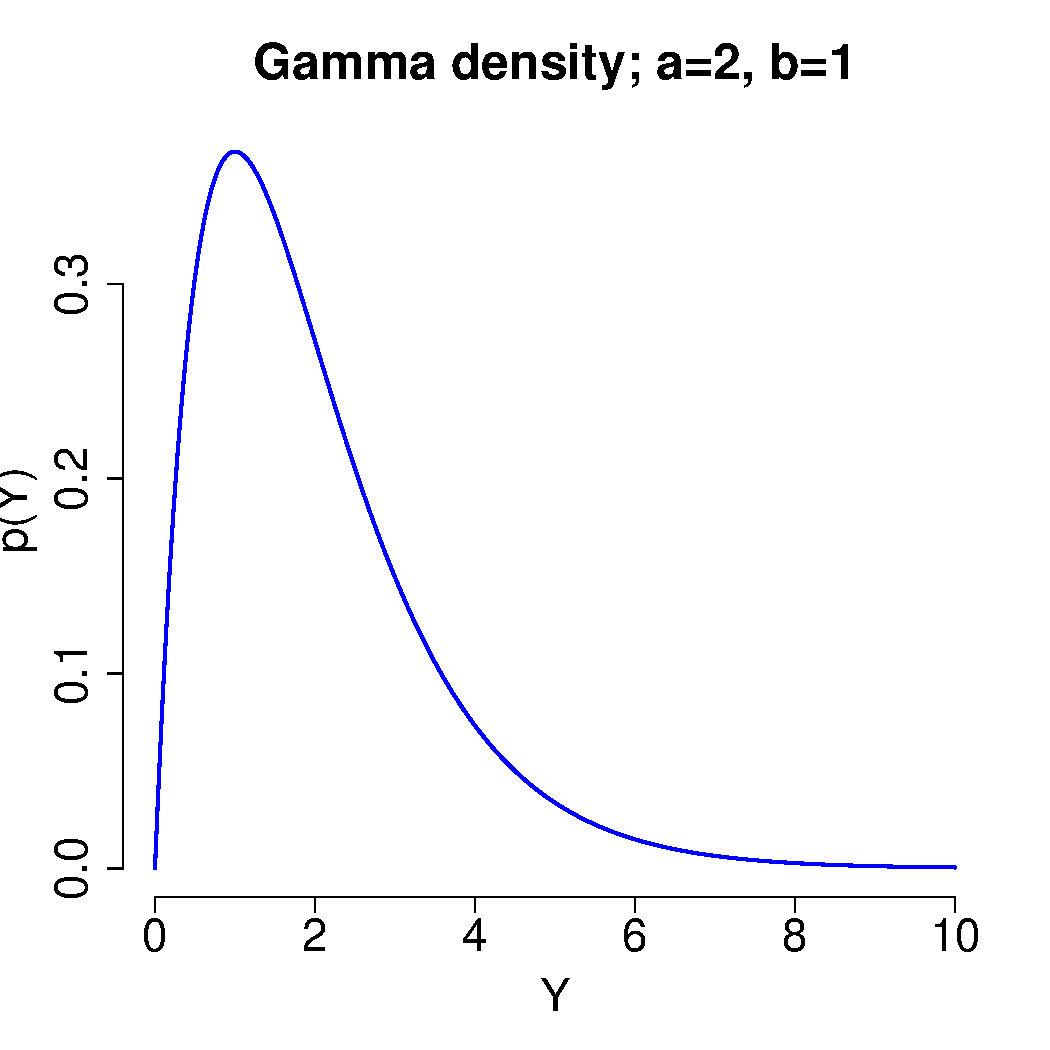
\includegraphics[width=0.33\textwidth]{../../figures/gamma_pdf}
		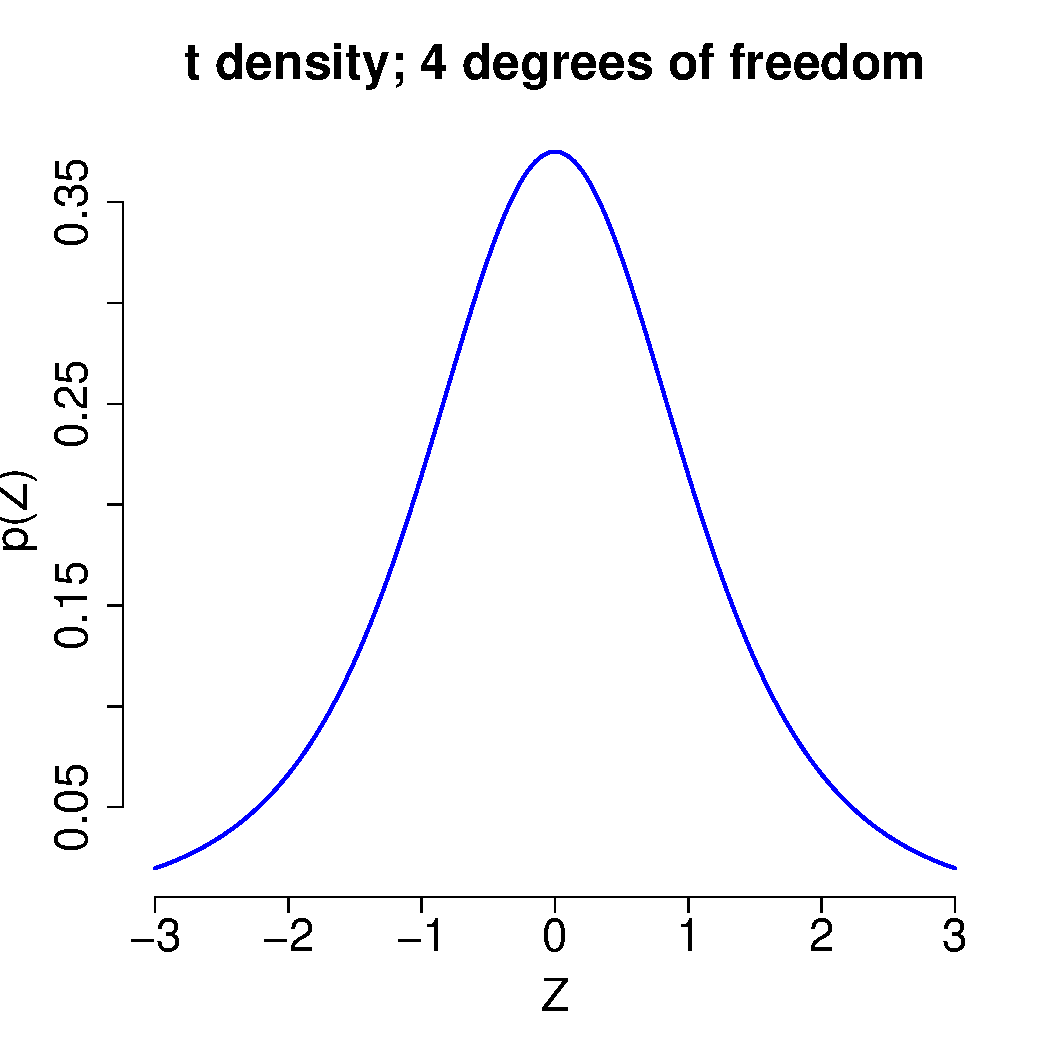
\includegraphics[width=0.33\textwidth]{../../figures/t_pdf}
	\end{center}
\end{frame}


\section{Current work}
%A little bit of Bayesian theory and description of python modeling

\begin{frame}{The surprise model}
	\begin{itemize}
		\item $Y \sim \text{Normal}(m, p)$ Where $m$ is the mean and $p$ is the precision.
		\item $m \sim \text{Normal}(\mu, p)$
		\item $p \sim \text{Gamma}(\alpha, \beta)$
	\end{itemize}
\end{frame}

\section{Value of the work}
%Simulation study, field data


\section{Future work}
%So, so much of it.


\end{document}